%%%%%%%%%%%%%%%%%%%%%%%%%%%%%%%%%%%%%%%%%
% Topological Data Analysis \& Image Classification
% Version 1.0 (20211125)
%
% Author: River Reger
% e-mail: river.reger@gmail.com
%%%%%%%%%%%%%%%%%%%%%%%%%%%%%%%%%%%%%%%%%

%----------------------------------------------------------------------------------------
%	PACKAGES AND THEMES
%----------------------------------------------------------------------------------------
\documentclass[10pt]{beamer}
\mode<presentation> {
\usetheme{Frankfurt}
\usecolortheme{beaver}
\setbeamertemplate{navigation symbols}{} % To remove the navigation symbols from the bottom of all slides
}
%==============================================================================
% Packages
%==============================================================================
\usepackage{graphicx} % Allows including images
\usepackage{booktabs} % Allows the use of \toprule, \midrule and \bottomrule in tables
\usepackage{bbm}
\usepackage{textpos}
\usepackage{tikz}
%==============================================================================
% Theorem formatting commands.
%==============================================================================
\theoremstyle{plain}
\newtheorem{thm}{Theorem}
\newtheorem{axiom}{Axiom}
\newtheorem{prop}{Proposition}
\newtheorem{cor}{Corollary}
\newtheorem{conj}{Conjecture}
\newtheorem{rul}{Rule}
\newtheorem*{thm*}{Theorem}
\newtheorem*{lemma*}{Lemma}
\newtheorem*{prop*}{Proposition}
\newtheorem*{cor*}{Corollary}
\newtheorem*{conj*}{Conjecture}

\theoremstyle{definition}
\newtheorem{defn}{Definition}
\newtheorem{ex}{Example}
\newtheorem{pr}{Problem}[section]
\newtheorem{soln}{Solution}[section]
\newtheorem{alg}[thm]{Algorithm}
\newtheorem{ques}[thm]{Question}

\theoremstyle{remark}
\newtheorem*{rmk}{Remark}
\newtheorem*{obs}{Observation}

%==============================================================================
% Blackboard Letters
%==============================================================================
%\newcommand{\aa}{\mathbb{A}}
\newcommand{\bb}{\mathbb{B}}
\newcommand{\cc}{\mathbb{C}}
\newcommand{\dd}{\mathbb{D}}
\newcommand{\ee}{\mathbb{E}}
\newcommand{\ff}{\mathbb{F}}
%\newcommand{\gg}{\mathbb{G}}
\newcommand{\hh}{\mathbb{H}}
\newcommand{\ii}{\mathbb{I}}
\newcommand{\jj}{\mathbb{J}}
\newcommand{\kk}{\mathbb{K}}
%\newcommand{\ll}{\mathbb{L}}
\newcommand{\mm}{\mathbb{M}}
\newcommand{\nn}{\mathbb{N}}
\newcommand{\oo}{\mathbb{O}}
\newcommand{\pp}{\mathbb{P}}
\newcommand{\qq}{\mathbb{Q}}
\newcommand{\rr}{\mathbb{R}}
%\newcommand{\ss}{\mathbb{S}}
%\newcommand{\tt}{\mathbb{T}}
\newcommand{\uu}{\mathbb{U}}
\newcommand{\vv}{\mathbb{V}}
\newcommand{\ww}{\mathbb{W}}
\newcommand{\xx}{\mathbb{X}}
\newcommand{\yy}{\mathbb{Y}}
\newcommand{\zz}{\mathbb{Z}}

%==============================================================================
%Caligraphics
%==============================================================================
\newcommand{\cA}{\mathcal{A}}
\newcommand{\cB}{\mathcal{B}}
\newcommand{\cC}{\mathcal{C}}
\newcommand{\cD}{\mathcal{D}}
\newcommand{\cE}{\mathcal{E}}
\newcommand{\cF}{\mathcal{F}}
\newcommand{\cG}{\mathcal{G}}
\newcommand{\cH}{\mathcal{H}}
\newcommand{\cI}{\mathcal{I}}
\newcommand{\cJ}{\mathcal{J}}
\newcommand{\cK}{\mathcal{K}}
\newcommand{\cL}{\mathcal{L}}
\newcommand{\cM}{\mathcal{M}}
\newcommand{\cN}{\mathcal{N}}
\newcommand{\cO}{\mathcal{O}}
\newcommand{\cP}{\mathcal{P}}
\newcommand{\cQ}{\mathcal{Q}}
\newcommand{\cR}{\mathcal{R}}
\newcommand{\cS}{\mathcal{S}}
\newcommand{\cT}{\mathcal{T}}
\newcommand{\cU}{\mathcal{U}}
\newcommand{\cV}{\mathcal{V}}
\newcommand{\cW}{\mathcal{W}}
\newcommand{\cX}{\mathcal{X}}
\newcommand{\cY}{\mathcal{Y}}
\newcommand{\cZ}{\mathcal{Z}}
\newcommand{\ca}{\mathcal{a}}

%==============================================================================
% Custom Commands
%==============================================================================
% \tbar{s}  -   Put a bar over a text character s.
\makeatletter
\newcommand*{\tbar}[1]{$\bar{\hbox{#1}}\m@th$}
\makeatother

% $\restr{f}{A}$  -   Restriction of function f to set A.
\newcommand\restr[2]{{% we make the whole thing an ordinary symbol
  \left.\kern-\nulldelimiterspace % automatically resize the bar with \right
  #1 % the function
  \vphantom{\big|} % pretend it's a little taller at normal size
  \right|_{#2} % this is the delimiter
  }}
		
%==============================================================================
% Custom Operators
%==============================================================================	
\DeclareMathOperator{\id}{id}
\newcommand{\Mod}[1]{\ (\mathrm{mod}\ #1)}
\DeclareMathOperator{\Span}{span}
\DeclareMathOperator{\card}{card}
\DeclareMathOperator{\Int}{Int}

%----------------------------------------------------------------------------------------
%	TITLE PAGE
%----------------------------------------------------------------------------------------
\title[TDA for Image Classification]{Topological Data Analysis (TDA) for Image Classification}
\subtitle{Virtual}
\author[River Reger]{River Reger \\ \href{mailto:river.reger@gmail.com}{river.reger@gmail.com}}
\date{\small Technical Presentation \\ 2021 November 29} % Date, can be changed to a custom date

\begin{document}

\begin{frame}
\titlepage % Print the title page as the first slide
\end{frame}

\begin{frame}
\frametitle{Overview}
\tableofcontents
\end{frame}
%----------------------------------------------------------------------------------------
%	PRESENTATION SLIDES
%----------------------------------------------------------------------------------------
%================================================
\section{Introduction to TDA}
%================================================
	%----------------------------------------------
	\subsection{Mathematics of Machine Learning}
	%----------------------------------------------
		\begin{frame}
		\frametitle{Mathematics of Machine Learning: Problem Statement}
		
		\begin{definition}
			Given an ideal function $f: X\rightarrow Y$, which associates \textbf{data} in $X\neq\phi$ with \textbf{measurements} in $Y\neq\phi$,
			the problem of \textbf{supervised learning} is to \textbf{learn} a \textbf{target function} $\hat{f}:X\rightarrow Y$, which approximates $f$,
			using a finite sample $S=\{(x_i,f(x_i))\}_{i=1}^n$, a \textbf{training set}.
		\end{definition}

		\begin{itemize}
			\item When $Y$ is finite, we say that this is a \textbf{supervised classification problem},
			otherwise, we say this is a \textbf{supervised regression problem}.
			\medskip
			\item In practice we often encode $Y$ to be isomorphic to $\rr^n$ or $\zz_n$ for some $n\in\nn$.
			(e.g., if the possible measurements are ``red'' and ``not red'', we encode this as $Y=\{0,1\}$).
		\end{itemize}
		\end{frame}
		
		\begin{frame}
		\frametitle{Mathematics of Machine Learning: Generalization}
		
		\begin{itemize}
			\item There are infinitely many $\hat{f}$ for which $\hat{f}(x_i) = f(x_i)$ for all $x_i\in S$. 
			\medskip
			\item For the purpose of machine learning, we are more interested not in
			fitting $\hat{f}$ to $S$, but in generalizing $\hat{f}$ to $X$; i.e., approximating $f$ on $X$.
			\medskip
			\item For this reason, we often partition $S$ into two sets $S_{\text{train}}$ and $S_{\text{test}}$.
			\medskip
			\item We first find $\hat{f}$ which performs well on $S_{\text{train}}$, then we validate this on $S_{\text{test}}$.
			\medskip
			\item This does not guarantee accuracy on $X$. It is an open problem of research to establish useful conditions under
			which training and test set performance will generalize to the entire set $X$.
		\end{itemize}
		\end{frame}

		\begin{frame}
		\frametitle{Mathematics of Machine Learning: Hypothesis Space}
		\begin{itemize}
			\item The \textbf{hypothesis space} for the supervised learning problem is $\cH = \{f:X\rightarrow Y\}$.
			\medskip
			\item It is not computationally feasible to search over the space
			of all such functions for $f$, especially when the $X$ is infinite or extremely large. Instead we choose a class of target functions $\hat{H}$.
			\medskip
			\item Once a class of target functions has been selected, a \textbf{loss function} $J:\hat{\cH}\times \cH\rightarrow \rr$ is selected.
			\medskip
			\item A popular example of this is the mean squared error:
				$$J(\hat{f},f) = \frac{1}{n} \sum_{i=1}^n (f(x_i)-\hat{f}(x_i))^2.$$
			\item In the case where $Y=\{0,1\}$, a popular loss function is \textbf{logarithmic loss}:
				$$J(f,\hat{f}) = -f(x_i)\log(\hat{f}(x_i))+(1-f(x_i))\log(1-\hat{f}(x_i)).$$
		\end{itemize}
		\end{frame}

		\begin{frame}
		\frametitle{Mathematics of Machine Learning: Optimization}
		
			\begin{itemize}
			\item The task of learning $\hat{f}$ is to minimize $J$.
			\item There is copious literature on the subject of optimization and loss functions in a machine learning context.
			\item One of the most popular methods of optimization for machine learning is Adam, or adaptive moment estimation.
			\item It is beyond the scope of this talk to delve into the details of Adam.
			\item The selection of an optimization algorithm can impact the performance of machine learning significantly. 
			\item See details of Adam here: \url{https://arxiv.org/pdf/1412.6980.pdf}
			\end{itemize}
		\end{frame}
		
		\begin{frame}
		\frametitle{Mathematics of Machine Learning: Pipeline}
		\begin{itemize}
			\item Define the problem in terms of an ideal function $f$ and a dataset $S$.
			\medskip
			\item Select a target function class; i.e., $\hat{H}$.
			\medskip
			\item Select a loss function $J$; e.g., mean squared error.
			\medskip
			\item Select an optimization method; e.g., Adam.
			\medskip
			\item Learn $\hat{f}$ by optimizing $J$ over $S$ (i.e., implement the machine learning architecture design).
			\medskip
			\item Analyze the results usually with statistics-based methods such as area under curve (AUC) and iterate on the design.
		\end{itemize}
		
		Note: if enough computational resources are available, hyperparameter search can be used to automate some of the iteration.
		
		\end{frame}
	%----------------------------------------------
	\subsection{Topological Data Analysis Motivations}
	%----------------------------------------------	
		\begin{frame}
		\frametitle{Traditional Assumptions of Data Analytics}
		\begin{itemize}
			\item Qualitative information is required - we wish to classify data/datasets by describing global properties (i.e., features).
				\begin{itemize}
					\item Loss/error functions are quantitative in nature.
				\end{itemize}
			\item Metrics usually have no basis in physics (counterexample to this would be Physics-informed Neural Networks).
				\begin{itemize}
					\item Optimization of machine learning algorithms is sensitive to metric choice (e.g., mean squared error).
				\end{itemize}
			\item Coordinates are not usually natural (unlike state vector coordinates from physics).
				\begin{itemize}
					\item The representation of data matters significantly, especially in terms of coordinates (normalized data vs. raw data).
				\end{itemize}
			\item Preference of summaries over individual parameter selection.
				\begin{itemize}
					\item Parameter selection and hyperparameter search look for optimal parameters, but this is computationally expensive.
				\end{itemize}
		\end{itemize}
		\end{frame}
		
		\begin{frame}
		\frametitle{Topological Data Analysis}
		\begin{itemize}
			\item Qualitative information is required - we wish to classify data/datasets by describing global properties.
				\begin{itemize}
					\item Topology captures global qualitative information via connectivity information about
					the underlying surface (e.g., manifold) that data resides within.
				\end{itemize}
			\item Metrics usually have no basis in physics.
				\begin{itemize}
					\item Less sensitivity to metric choice in topology since spatial information is not dependent on true distance, but relative placement.
				\end{itemize}
			\item Coordinates are not usually natural.
				\begin{itemize}
					\item Topology is coordinate free by definition. We place topological structure on a coordinate space, but that structure is not the significant factor.
				\end{itemize}
			\item Preference of summaries over individual parameter selection.
				\begin{itemize}
					\item The powerhouse of topological data analysis is persistent homology, which looks at all possible parameter choices
					as a summary versus endlessly searching a large hyperparameter space.
				\end{itemize}
		\end{itemize}
		\end{frame}
	%----------------------------------------------
	\subsection{Basic Topological Structures}
	%----------------------------------------------
		\begin{frame}
		\frametitle{Spaces Under Study}
		
		\begin{defn}
		Let $X\neq\phi$ and $d:X\times X\rightarrow [0,\infty)$. Then $d$ is said to be a \textbf{metric} on $X$, and the pair
		$(X,d)$ a \textbf{metric space} if for all $x,y,z\in X$:
			\begin{enumerate}
				\item $d(x,y) = 0$ iff $x=y$
				\item $d(x,y) = d(y,x)$
				\item $d(x,z) \leq d(x,y) + d(y,z)$
			\end{enumerate}
		\end{defn}
		
		\begin{defn}
		Let $X\neq\phi$ and $\cT\subseteq X$. Then $\cT$ is a \textbf{topology} on $X$, and the pair $(X,\cT)$ is said to be a \textbf{topological space}, if
			\begin{enumerate}
				\item $X,\phi\in\cT$
				\item $\cT$ is closed under arbitrary unions
				\item $\cT$ is closed under finite intersections.
			\end{enumerate}
		The members of $\cT$ are said to be \textbf{open}.
		\end{defn}
		\end{frame}
		
		\begin{frame}
		\frametitle{Continuity}
		
		\begin{defn}
		Let $(X,\cT_X)$ and $(Y,\cT_Y)$ be topological spaces and $f:X\rightarrow Y$. Then $f$ is \textbf{continuous} at $x_0$ if for every $V(f(x))\in\cT_Y$, there exists $U(x)\in \cT_X$ such that $f(U)\subseteq V$.
		\end{defn}
		
		\begin{defn}
		Let $(X,d)$ be a metric space and $\epsilon>0$, then the open ball $B(x;\epsilon)=\{y: d(x,y)<\epsilon\}$
		\end{defn}
		
		\begin{defn}
		Let $(X,d)$ and $(Y,d_Y)$ be metric spaces. Then $f:X\rightarrow Y$ is continuous at $x_0\in X$ if for every
		$\epsilon>0$, there exists $\delta>0$ such that $f(B(x_0;\delta))\subseteq B(y;\epsilon)$.
		\end{defn}		
		\end{frame}
		
		\begin{frame}
		\frametitle{Point Clouds and Homeomorphism}
		
		\begin{defn}
		A \textbf{point cloud} is a finite metric space (i.e., $(X,d)$ such that $X=\{x_1,\ldots,x_n\}$). As such all datasets encoded in computers can be seen as mathematical point clouds.
		\end{defn}
		
		\begin{defn}
		Let $f:X\rightarrow Y$ be bicontinuous (continuous $f$ and $f^{-1}$). Then $f$ is a \textbf{homeomorphism} and we say $X$ is homeomorphic to $Y$; $X\cong Y$. If a property holds for $X$ and for any homeomorphism $f(X)$, then we say that property is a \textbf{topological invariant}.
		\end{defn}
		
		\begin{itemize}
			\item Since every dataset is a point cloud (i.e., a metric space), every dataset has a topology, dependent on the choice of metric.
			\item E.g., $32\times 32$ black and white images can be seen as lying in $\cM^{32\times 32}([0,1])$. We can endow this space
			with a metric (e.g., Euclidean distance), which makes it a point cloud. Since it is also a point cloud, it has an underlying topology.
			\item $\cM^{32\times 32}([0,1]) \cong [0,1]^{1024}$.
		\end{itemize}
		\end{frame}
	%----------------------------------------------
	\subsection{Algebraic Topology: Connectivity Information}
	%----------------------------------------------
		\begin{frame}
		\frametitle{Homotopy}
		
		\begin{definition}
			If $f,g:X\rightarrow Y$ are continuous, we say that they are \textbf{homotopic} if $H:X\times[0,1]\rightarrow Y$ is such that $H(x,0)=f(x)$
			and $H(x,1)=g(x)$. Furthermore, we say that $f:X\rightarrow Y$ is a \textbf{homotopy equivalence} if there exists $G:Y\rightarrow X$ such 
			that $f\circ g$ is homotopic to $\mathrm{id}_X$ and $g\circ f$ is homotopic to $\mathrm{id}_Y$. If $X$ is homotopy equivalent to $Y$ then 
			we say they are \textbf{homotopic} spaces.
		\end{definition}

		\begin{itemize}
			\item See \textit{Algebraic Topology} by Hatcher for a more thorough treatment of this topic.
			\item It is enough for us to note with some hand-waving that there is a group $H_k(X,A)$ for any commutative group $A$ and non-negative 
			integer $k$, such that when $X$ and $Y$ are homotopic, $H_k(X,A)$ is \textbf{isomorphic} (i.e., operation-preserving) to $H_k(Y,A)$. 
			\item We call $H_k(X,A)$ the \textbf{homotopy group} of $X$.
		\end{itemize}
		\end{frame}
		
		\begin{frame}
		\frametitle{Homotopy}
		With respect to $H_k(X,A)$:
		\begin{itemize}
			\item If we require $A$ to be a field, then $H_k(X,A)$ is a vector space.
			\item We denote the dimension of this vector space as $\beta_k(X,A)$, which will be referred to as the $k-$th Betti number.
			\item Informally, the $k-$th Betti number corresponds to the number of independent $k-$dimensional surfaces.
			\item If two spaces are homotopy equivalent, then all their Betti numbers are equal.
			\item The profound observation of TDA, is that data may be studied by studying the inherent independent $k-$dimensional surfaces.
			\item This structure is not one that has been engineered, but one that is inherent in the data's topological structure.
			\item Computationally, it is not feasible/efficient to compute $H_k(X,A)$.
		\end{itemize}
		\end{frame}

		\begin{frame}
		\frametitle{Homology}
		
		\begin{itemize}
			\item Homology is a computationally feasible analog for homotopy equivalences.
			\item The rigorous definition of homology for general topology relies on infinitely generate modules over $\zz$.
			\item This definition is not useful from a data analytics perspective because it is computationally impossible to guarantee
			we could feasibly compute an approximation in general.
			\item However, using a simple combinatorial structure called \textbf{simplicial complexes}, we can determine the homology of a given point cloud efficiently.
			\item We will see that we can actually extract Betti numbers from simplicial complexes.
		\end{itemize}
		\end{frame}
			
		\begin{frame}
		\frametitle{Complexes}
		\begin{defn}
		An \textbf{abstract simplicial complex} is a pair $(V,\Sigma)$ where $V$ is finite and $\Sigma$ is a family of non-empty subsets of $V$ such that:
		$$\sigma\in\Sigma \;\;\;\text{and}\;\;\; \tau\subseteq\sigma \;\;\;\text{implies}\;\;\; \tau\in\Sigma$$
		\end{defn}
		
		\begin{itemize}
			\item Intuitively, simplicial complexes express a space of points, segments, triangles, tetrahedrons, and their higher dimensional analogues.
			\item These provide a particularly simple way to approximate topological spaces (in terms of homotopy/homology).
			\item Simplicial complexes admit a topology as well as an associated vector space (beyond the scope for this talk).
			\item It is computationally efficient to determine the homology of simplicial complexes compared to the original topological space.
			\item Rigorously, this is done by computing $H_k^{\text{simp}}(X,\zz)$, associated with the simplicial complex $X=(V,\Sigma)$.
			\item $H_k^{\text{simp}}(X,\zz)$ is isomorphic to the homology of $X$, which can be generate for a given point cloud.
			\item See Gunnar Carlsson's ``Topology and Data.''
		\end{itemize}
		
		\end{frame}
			
		\begin{frame}
		\frametitle{Persistent Homology}
		\begin{itemize}
			\item In order to guarantee that the homology of the point cloud $X$ corresponds with the homology of a simplicial complex $(V,\Sigma)$
			is to build this complex in such a way that there is a homotopy equivalence between $X$ and $(V,\Sigma)$.
			\item One such complex is the Vietoris-Rips simplicial complex.
			\end{itemize}
			
			\begin{defn}			
			For a metric space $(X,d)$, the Vietoris-Rips simplicial complex associated with $\epsilon>0$, whose vertex set is $X$ and where $\{x_0,\ldots,x_k\}$ spans a $k-$dimensional subset iff $d(x_i,x_j)\leq\epsilon$ for all $i,j\leq k$.
			\end{defn}
			
			By varying $\epsilon$, we can study the homology of a point cloud at varying scales. We thus do not tie ourselves to one homology, but study the \textbf{persistent homologies} across sufficient choices of $\epsilon$ to summarize the topological information within the data.
		\end{frame}
		
				\begin{frame}
		\frametitle{VR Complexes}
		
				\begin{figure}
				\centering
				\includegraphics[scale=0.5]{images/complex.png}
				\caption{Sample simplicial complex structure using the Vietoris-Rips construction. As $\epsilon$ varies, the homology groups of the complex change.}
		\end{figure}
		\end{frame}
		
	%----------------------------------------------
	\subsection{Persistent Homology Representations}
	%----------------------------------------------
		\begin{frame}
		\frametitle{Persistence Diagrams}
		\begin{itemize}
			\item This is a representation of the persistent homology information.
			\item Persistence Diagrams (PDs) can be encoded in terms of two-dimensional vectors $(b_i,d_i)$, where $b_i$ is the birth and $d_i$ is the death of the $i^{\text{th}}$ homology feature.
			\item PDs have a natural metric associated with them called the \textbf{bottleneck distance}, which is numerically stable and computationally efficient to compute.
			\item We often design algorithms for TDA on PDs under the bottleneck distance.
		\end{itemize}
		
		\end{frame}
		
		\begin{frame}
		\frametitle{Persistence Diagram Example}
		
						\begin{figure}
				\centering
				\includegraphics[scale=0.5]{images/pd.png}
				\caption{Sample persistence diagram visualized in $\rr^n$ as a set of (birth,death) pairs.}
		\end{figure}
		\end{frame}
		
		\begin{frame}
		\frametitle{Persistence Barcodes}
		\begin{itemize}
			\item Persistent Barcodes are an alternative representation to PDs, mostly used for visualization.
			\item Instead of considering $(b_i,d_i)$ pairs as points, we look at them as segments/intervals and organize them with respect to the $k^{\text{th}}$ Betti number ($y$-axis).
		\end{itemize}
		
						\begin{figure}
				\centering
				\includegraphics[scale=0.5]{images/barcode.png}
				\caption{Sample barcode. As $\epsilon$ varies, the homology groups of the complex change and this is captured by line segments representing $[$birth, death$]$ intervals.}
		\end{figure}
		
		
		\end{frame}
		
		\begin{frame}
		\frametitle{Persistence Images}
		\begin{itemize}
			\item Persistence Images (PIs) provide a vector representation of PDs stable with respect to input noise, which are efficient to compute, and whose resolution can be adjusted.
			\item The user makes three choices for this representation:
			\begin{itemize}
				\item Resolution of the output PI.
				\item Probability distribution which affects noise stability (e.g., Gaussian, Rayleigh).
				\item Weighting function, which controls the relative importance of persistence coordinates (e.g., sigmoidal functions).
			\end{itemize}
			\item PIs lend themselves to being studied under traditional image processing techniques as well as convolutional neural networks.
		\end{itemize}
		
		\end{frame}
		
		\begin{frame}
		\frametitle{Persistence Image Example}
		
						\begin{figure}
				\centering
				\includegraphics[scale=0.35]{images/persimg.png}
				\caption{Sample persistence image pipeline from PD to Persistence Surface to PI at varying resolutions.}
		\end{figure}
		\end{frame}
		
		\begin{frame}
		\frametitle{Open Source Tools for Computing Persistent Homology}
		\begin{itemize}
			\item There have been a number of open source software packages developed for the efficient computation of persistent homology of data.
			\item These have been developed mostly by academic mathematicians in Python, C++, R, and Julia.
			\item Most popular ones include dionysus, scikit-tda, gudhi, ripser, and mapper.
			\item A full list of these tools has been compiled by \href{https://www.math.colostate.edu/~adams/advising/appliedTopologySoftware/}{Henry Adams}.
		\end{itemize}
		
		\end{frame}
%================================================
\section{Iris Dataset}
%================================================
	%----------------------------------------------
	\subsection{Problem and Approach}
	%----------------------------------------------
		\begin{frame}
		\frametitle{Iris Data Classification}
		
		\begin{itemize}
			\item Very small dataset (150 points with 4 features, 3 labels, balanced).
			\item 4 features: sepal length/width (cm), petal length/width (cm) 
			\item 3 classes: setosa, versicolor, and virginica
			\item Very simple and computationally easy, which makes it ideal for quick sanity checks.
			\item Analsis Tools Considered:
				\begin{itemize}
					\item PCA Clustering (qualitative)
					\item K Nearest Neighbor Classifier Accuracy (quantitative)
					\item K Nearest Neighbor Confusion Matrix (quantitative)
					\item Persistence Diagrams (qualitative)
					\item Bottleneck Distance Matrix (quantitative)
				\end{itemize}
		\end{itemize}
		
		\end{frame}
		
	%----------------------------------------------
	\subsection{Results}
	%----------------------------------------------
		
		\begin{frame}
		\frametitle{PCA Clustering}
		
		\begin{figure}
				\centering
				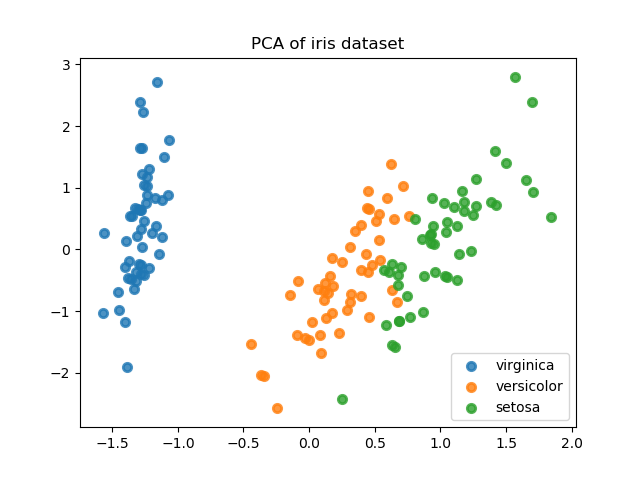
\includegraphics[scale=0.5]{images/iris_PCA.png}
				\caption{PCA Clustering of the Iris Dataset. Visually, we can see that the setosa label has high separability from versicolor and virginica, which are much closer after PCA.}
		\end{figure}
		
		\end{frame}
		
		\begin{frame}
			\frametitle{K Nearest Neighbors Classifier}
			
			\begin{itemize}
				\item Pre-processing:
				\begin{itemize}
					\item We split the data into a 30\% train and 70\% test sets and keep the data balanced.
					\item We also shuffle the data.
					\item We scale the data such that it is within $(0,1)$ using a min-max scaler.
				\end{itemize}
				\item The function class we consider is trivial since it is dependent only on the training data given.
				\item We can view this as a weighting function that weights the $k$-nearest points to the input with $\frac{1}{k}$ and all other points $0$.
				\item Classification Accuracy: 83 percent
				\item Training Accuracy: 91 percent
			\end{itemize}
		\end{frame}
		
		\begin{frame}
			\frametitle{Confusion Matrix for Iris Data}
			
			\begin{figure}
				\centering
				\includegraphics[scale=0.5]{images/confusion_matrix_iris.png}
				\caption{Confusion Matrix of Iris Data. We see that setosa is classified perfectly, while versicolor and virginica have some errors in classification.}
		\end{figure}
		\end{frame}
		
		\begin{frame}
		\frametitle{Persistence Diagrams of Iris Features: Setosa}
		
		\begin{figure}
				\centering
				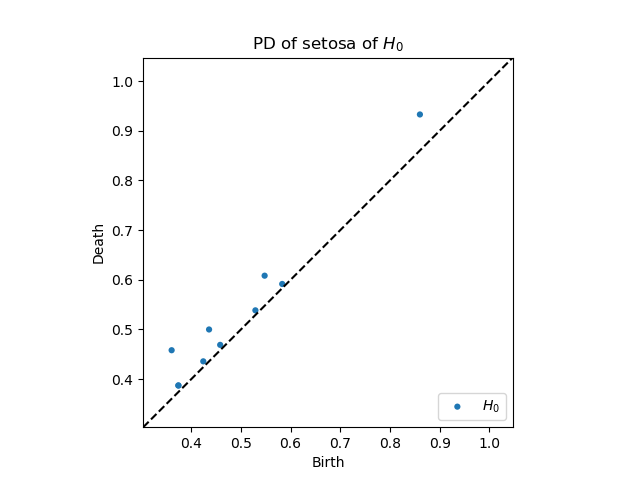
\includegraphics[scale=0.5]{images/PD_H0_setosa.png}
				\caption{Persistence Diagram for Setosa}
		\end{figure}
		\end{frame}

		\begin{frame}
		\frametitle{Persistence Diagrams of Iris Features: Versicolor}
		
		\begin{figure}
				\centering
				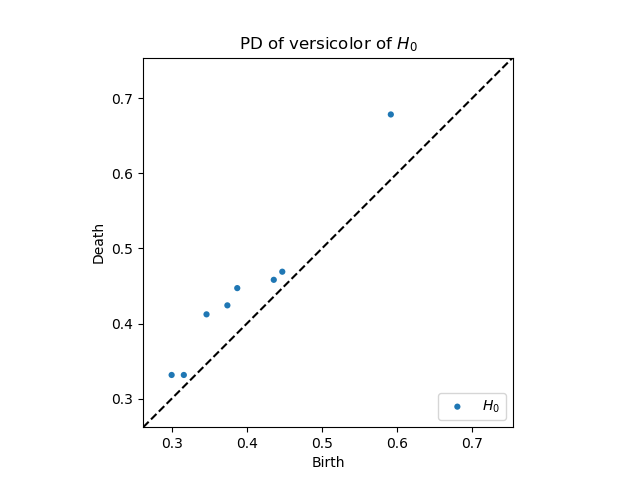
\includegraphics[scale=0.5]{images/PD_H0_versicolor.png}
				\caption{Persistence Diagram for Versicolor.}
		\end{figure}
		\end{frame}
		
		
				\begin{frame}
		\frametitle{Persistence Diagrams of Iris Features: Virginica}
		
		\begin{figure}
				\centering
				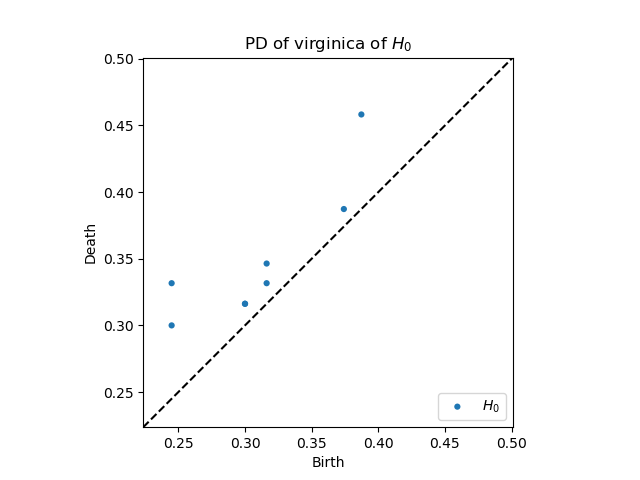
\includegraphics[scale=0.5]{images/PD_H0_virginica.png}
				\caption{Persistence Diagram for Virginica.}
		\end{figure}
		\end{frame}
		
		\begin{frame}
		\frametitle{Pairwise Bottleneck Distances}
		
		\begin{itemize}
			\item The bottleneck distances for each of the iris varieties:
				\begin{itemize}
					\item With themselves: 0 (control)
					\item Setosa, Virginica: 0.04335675
					\item Setosa, Versicolor: 0.04335675
					\item Virginica, Versicolor: 0.04331252
				\end{itemize}
		\end{itemize}
		
		A downside to the Bottleneck Distance as a measure is that quantitatively it can be hard to distinguish for simple data what a good distance is.
		\end{frame}
		
%================================================
\section{NIST Digits Dataset}
%================================================
	%---------------------------------------------
	\subsection{Problem and Approach}
	%----------------------------------------------
	\begin{frame}
		\frametitle{NIST Data Classification}
		
		\begin{itemize}
			\item Small dataset (1797 points with 64 features, 10 labels, balanced).
			\item 64 features: $8\times 8$ images with pixels in the range $[0,16]$. 
			\item 10 classes: 0, 1, 2, 3, 4, 5, 6, 7, 8, 9
			\item Simple and computationally able to run locally, which makes it ideal for proof-of-concept on short timelines where image analysis is needed quickly.
			\item Analsis Tools Considered:
				\begin{itemize}
					\item PCA Clustering (qualitative)
					\item K Nearest Neighbor Classifier Accuracy (quantitative)
					\item K Nearest Neighbor Confusion Matrix (quantitative)
					\item Persistence Diagrams (qualitative)
					\item Bottleneck Distance Matrix (quantitative)
				\end{itemize}
		\end{itemize}
		
		\end{frame}
		
		
	%----------------------------------------------
	\subsection{Results}
	%----------------------------------------------
		
		\begin{frame}
		\frametitle{PCA Clustering}
		
		\begin{figure}
				\centering
				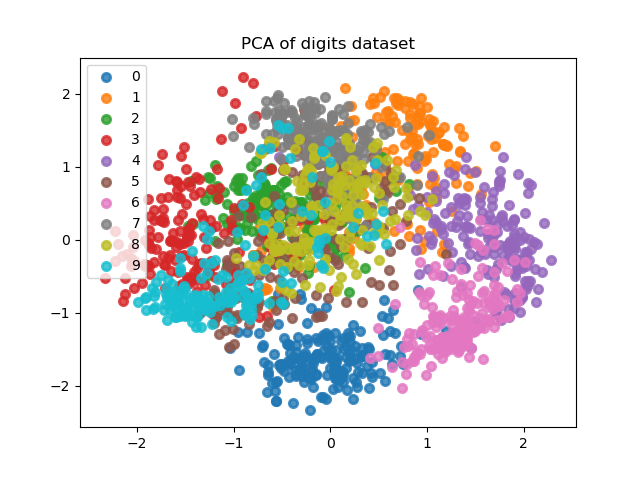
\includegraphics[scale=0.5]{images/digits_PCA.png}
				\caption{PCA Clustering of the NIST Digits Dataset. Visually, we can see that there is some clustering, but the data has a pretty high degree of similarity even after PCA.}
		\end{figure}
		
		\end{frame}
		
		\begin{frame}
			\frametitle{K Nearest Neighbors Classifier}
			
			\begin{itemize}
				\item Pre-processing:
				\begin{itemize}
					\item We split the data into a 30\% train and 70\% test sets and keep the data balanced.
					\item We also shuffle the data.
					\item We scale the data such that it is within $(0,1)$ using a min-max scaler.
				\end{itemize}
				\item The function class we consider is trivial since it is dependent only on the training data given.
				\item We can view this as a weighting function that weights the $k$-nearest points to the input with $\frac{1}{k}$ and all other points $0$.
				\item Classification Accuracy: 76 percent
				\item Training Accuracy: 83 percent
			\end{itemize}
		\end{frame}
		
		\begin{frame}
			\frametitle{Confusion Matrix for Digits Data}
			
			\begin{figure}
				\centering
				\includegraphics[scale=0.5]{images/confusion_matrix_digits.png}
				\caption{Confusion Matrix of Digit Data. We see many interesting artifacts: 0's, 4's, and 6's are classified nicely, 1's have some confusion with 7's (vice versa), 2's with 5's, 3's with 9's, 5's with 8's, 8's with 2's and 5's, and 9's with 1's and 3's.}
		\end{figure}
		\end{frame}
		
		\begin{frame}
		\frametitle{Persistence Images of Digits: 0's}
		
		\begin{figure}
				\centering
				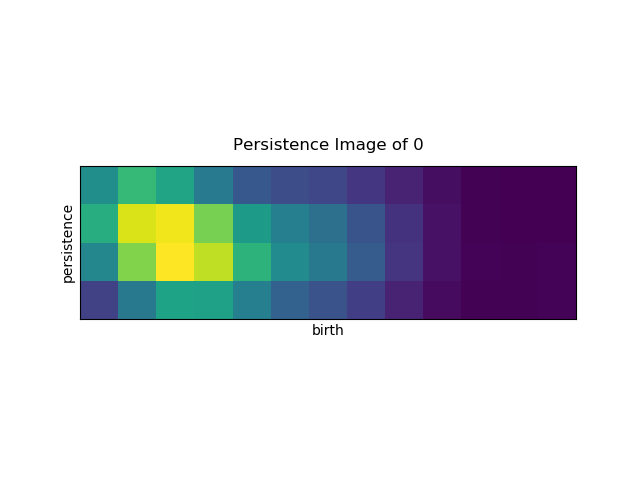
\includegraphics[scale=0.5]{images/PI_H0_0.png}
				\caption{Persistence Image for 0.}
		\end{figure}
		\end{frame}

		\begin{frame}
		\frametitle{Persistence Images of Digits: 0's}
		
		\begin{figure}
				\centering
				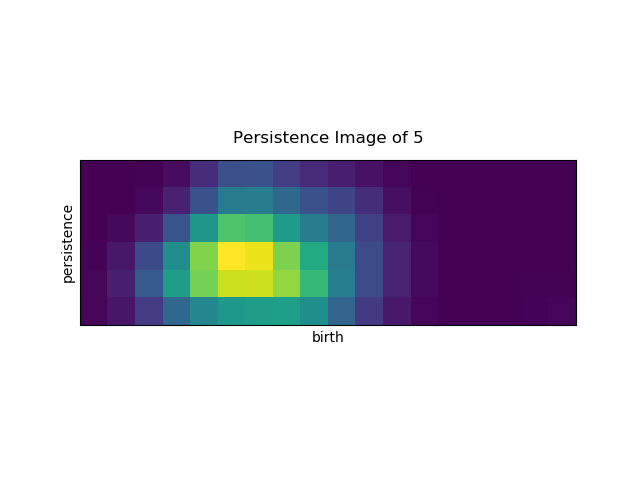
\includegraphics[scale=0.5]{images/PI_H0_5.png}
				\caption{Persistence Image for 5.}
		\end{figure}
		\end{frame}
		
		
				\begin{frame}
		\frametitle{Persistence Images of Digits: 8's}
		
		\begin{figure}
				\centering
				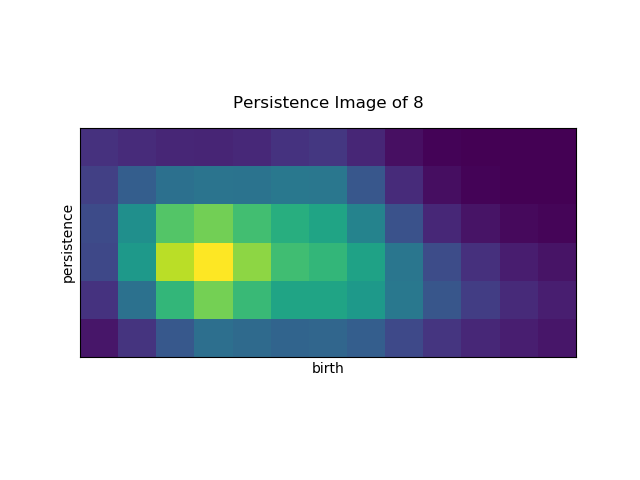
\includegraphics[scale=0.4]{images/PI_H0_8.png}
				\caption{Persistence Image for 8.}
		\end{figure}
		\end{frame}
		
				\begin{frame}
		\frametitle{Persistence Diagram of Digits: 0's, 5's, \& 8's}
		
		\begin{figure}
				\centering
				\includegraphics[scale=0.35]{images/pd058.png}
				\caption{Persistence Image for 0, 5, 8. Notice the birth/death are similar for 5 and 8 versus 0.}
		\end{figure}
		\end{frame}
		
		
		
		
		\begin{frame}
		\frametitle{Pairwise Bottleneck Distances}
		
		\begin{itemize}
			\item The bottleneck distances:
				\begin{itemize}
					\item With themselves: 0 (control)
					\item 0, 5: 2.56941795
					\item 0, 8: 2.21272278
					\item 5, 8: 2.11571217 
				\end{itemize}
		\end{itemize}
		
		A downside to the Bottleneck Distance as a measure is that quantitatively it can be hard to distinguish for simple data what a good distance is.
		\end{frame}
%================================================
\section{Breast Cancer Dataset}
%================================================
	%----------------------------------------------
	\subsection{Problem and Approach}
	%----------------------------------------------
		\begin{frame}
		\frametitle{Breast Cancer Data Classification}
		
		\begin{itemize}
			\item Small dataset (569 points with 30 features, 2 labels, nearly balanced).
			\item 30 features: numeric such as radius, texture, concavity, etc. 
			\item 2 classes: benign and malignant
			\item Very simple and computationally easy, but with far more dynamic feature set.
			\item Analsis Tools Considered:
				\begin{itemize}
					\item PCA Clustering (qualitative)
					\item K Nearest Neighbor Classifier Accuracy (quantitative)
					\item K Nearest Neighbor Confusion Matrix (quantitative)
					\item Persistence Diagrams (qualitative)
					\item Bottleneck Distance Matrix (quantitative)
				\end{itemize}
		\end{itemize}
		
		\end{frame}
		
		%----------------------------------------------
	\subsection{Results}
	%----------------------------------------------
		
		\begin{frame}
		\frametitle{PCA Clustering}
		
		\begin{figure}
				\centering
				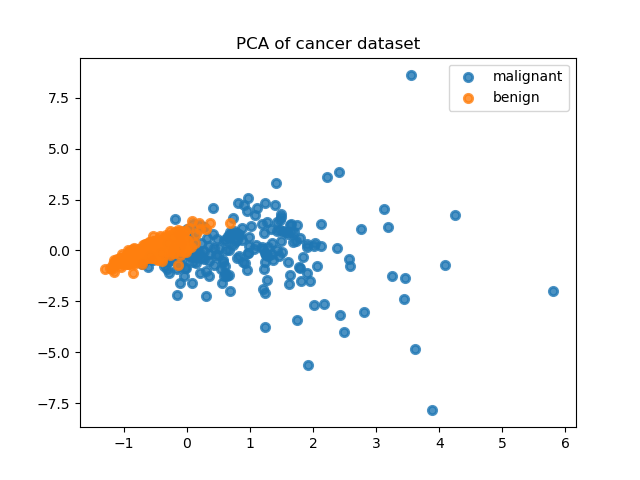
\includegraphics[scale=0.5]{images/cancer_PCA.png}
				\caption{PCA Clustering of the Breast Cancer Dataset. Visually, we can see that there is some separation, but the data lies close even after PCA.}
		\end{figure}
		
		\end{frame}
		
		\begin{frame}
			\frametitle{K Nearest Neighbors Classifier}
			
			\begin{itemize}
				\item Pre-processing:
				\begin{itemize}
					\item We split the data into a 30\% train and 70\% test sets and keep the data balanced.
					\item We also shuffle the data.
					\item We scale the data such that it is within $(0,1)$ using a min-max scaler.
				\end{itemize}
				\item The function class we consider is trivial since it is dependent only on the training data given.
				\item We can view this as a weighting function that weights the $k$-nearest points to the input with $\frac{1}{k}$ and all other points $0$.
				\item Classification Accuracy: 91 percent
				\item Training Accuracy: 94 percent
			\end{itemize}
		\end{frame}
		
		\begin{frame}
			\frametitle{Confusion Matrix for Cancer Data}
			
			\begin{figure}
				\centering
				\includegraphics[scale=0.5]{images/confusion_matrix_cancer.png}
				\caption{Confusion Matrix of Cancer Data. The data is pretty nicely classified in this binary case.}
		\end{figure}
		\end{frame}
		
		
		
		\begin{frame}
		\frametitle{Persistence Diagrams of Digits: Benign}
		
		\begin{figure}
				\centering
				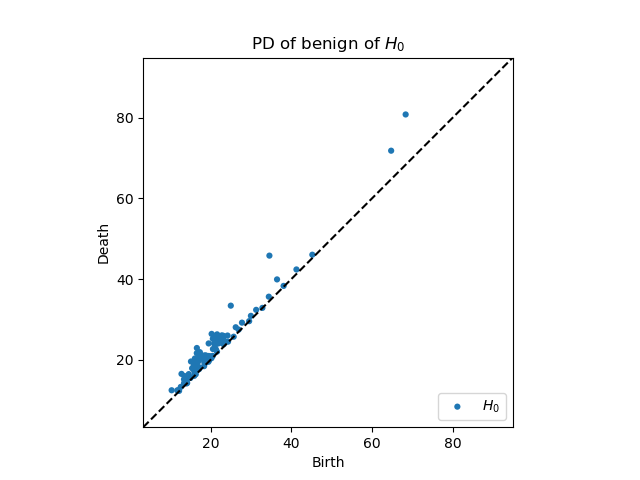
\includegraphics[scale=0.5]{images/PD_H0_benign.png}
				\caption{Persistence Diagram for Benign.}
		\end{figure}
		\end{frame}

		\begin{frame}
		\frametitle{Persistence Diagrams of Digits: Malignant}
		
		\begin{figure}
				\centering
				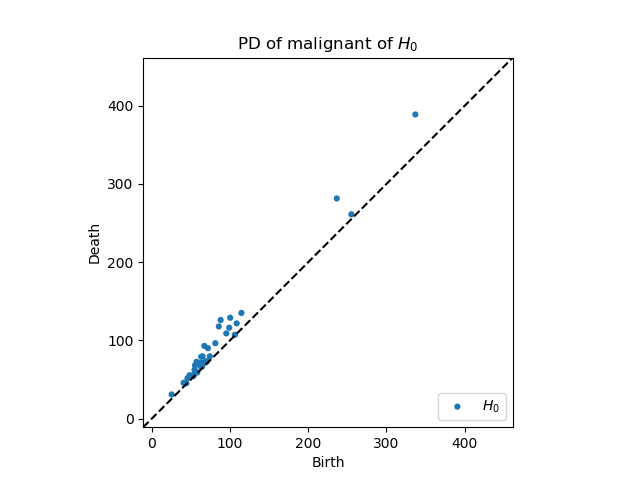
\includegraphics[scale=0.5]{images/PD_H0_malignant.png}
				\caption{Persistence Diagram for Malignant.}
		\end{figure}
		\end{frame}
		
		
		\begin{frame}
		\frametitle{Persistence Images of Digits: Benign}
		
		\begin{figure}
				\centering
				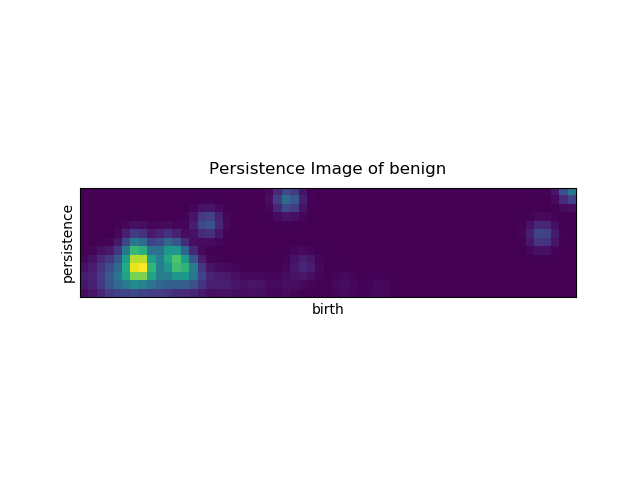
\includegraphics[scale=0.5]{images/PI_H0_benign.png}
				\caption{Persistence Image for Benign.}
		\end{figure}
		\end{frame}

		\begin{frame}
		\frametitle{Persistence Images of Digits: Malignant}
		
		\begin{figure}
				\centering
				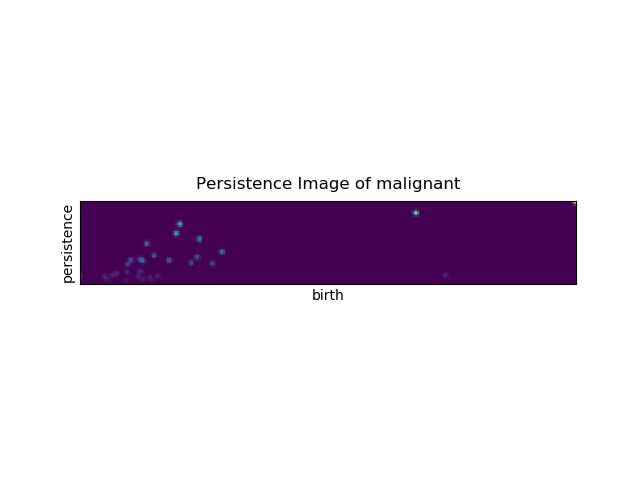
\includegraphics[scale=0.5]{images/PI_H0_malignant.png}
				\caption{Persistence Image for Malignant.}
		\end{figure}
		\end{frame}
		
		
		\begin{frame}
		\frametitle{Pairwise Bottleneck Distances}
		
		\begin{itemize}
			\item The bottleneck distances:
				\begin{itemize}
					\item With themselves: 0 (control)
					\item Benign, Malignant: 25.95355225
				\end{itemize}
		\end{itemize}
		
		A downside to the Bottleneck Distance as a measure is that quantitatively it can be hard to distinguish for simple data what a good distance is. In the binary case, unless you are comparing for hyperparameter search, this metric is close to useless.
		\end{frame}


%================================================
\section{Conclusions \& Questions}
%================================================
	\begin{frame}
			\frametitle{Conclusions}
			\begin{itemize}
				\item Traditional Data Analysis has seen great progress over the past decade due to the copious amounts of data
				available paired with ever increasing availability of high performance computing resources.
				\item TDA offers new and rigorous tools from mathematics for analyzing datasets at a global scale.
				\item As seen in the simple dataset examples, differences in data can be explained by the inherent homology information that is encoded within the dataset.
				\item This is a unique tool that can be added to data scientists' toolboxes for more detailed analysis of the underlying shape of data.
				\item The bottleneck metric must be used with caution as an actual scoring metric.
				\item The analysis from TDA tends to be less quantitative and more qualitative.
			\end{itemize}
	\end{frame}
		
	\begin{frame}
		\frametitle{Future Work}
		
		\begin{itemize}
			\item Since we can extract vectors and images as topological information, more work is needed on the practical meaningfulness of these features under traditional techniques including:
				\begin{itemize}
					\item Convolutional Neural Networks (CNNs) on Persistence Images
					\item Image Segmentation (noise/signal separation) on PIs.
					\item Support Vector Machines (SVMs) and other classical ML algorithms using persistence diagrams as vector sets.
				\end{itemize}
			\item There is a large gap in academia and practice in modalities beyond RGB images or small numerical vectors. Particular areas of interest could include:
				\begin{itemize}
					\item Non-image based data (radar waveforms, GDELT text-based data, sentiment analysis, etc.)
					\item Imagery: SAR (especially 3D SAR), HSI, MWIR, LWIR, Lidar
					\item Military messaging systems (Link-16 messages), scenario data (laydown parameters)
					\item Cybersecurity threat analysis
				\end{itemize}
		\end{itemize}
	\end{frame}

	\begin{frame}
		\Huge{\centerline{Questions?}}
	\end{frame}
\end{document} 